\par En este último ejercicio vamos a poner a prueba las distintas heurísticas y metaheurísticas planteadas en los ejercicios previos con una serie de casos y compararemos su rendimiento y la calidad de la solución. La idea principal de esta sección es sacar conclusiones sobre en qué aspectos un algoritmo se desempeña y en qué aspectos no consideramos beneficioso utilizarlo.

\par Antes de comenzar, definiremos una numeración para los programas. Esto hará más fácil la explicación y la referencia a cada programa.

\begin{itemize}
	\item \textbf{Programa 1}: Programa visto en el ejercicio 1, basando en un algoritmo de backtracking. Genera una solución exacta.
	\item \textbf{Programa 2}: Programa visto en el ejercicio 2, implementación de un algoritmo basado en una heurística golosa.
	\item \textbf{Programa 3}: Programa visto en el ejercicio 3, implementación de un algoritmo basado en una heurística de búsqueda local.
	\item \textbf{Programa 4}: Programa visto en el ejercicio 4, implementación de un algoritmo basado en una metheurística que busca mejorar las soluciones dadas por la heurística de búsqueda local (programa 3).
\end{itemize}

\subsection{Generación de casos}

\par Para generar los casos utilizamos un script que recibe la cantidad de nodos del tipo gimnasio, la cantidad de nodos del tipo parada y la capacidad de la mochila. Luego, en base a estos datos, genera un caso de entrada al problema. Tanto la ubicación de los nodos como las pociones necesarias para matar a un gimnasio son generados de forma aleatoria dentro de un rango seteado manualmente.

\par Para el experimento se generaron casos que van desde 2 nodos hasta 3000. Se fué aumentando esta cantidad de nodos dependiendo de la cantidad actual, para generar más esparcimiento con cantidades más grandes. Por ejemplo, de 5 nodos se pasó a 6, pero de 155 nodos se pasó a 159, mientras que de 1402 se pasó a 1438.

\subsection{Ejecución del experimento}

\par Debido a los tiempos de ejecución de cada programa, se decidió establecer rangos en los cuales se correrán cada programa. Por ejemplo, se sabe que el programa 1 tiene una complejidad elevada y por eso se diseñan heurísticas que den soluciones cercanas en menos tiempo. Por esto el programa será ejecutado para casos de entrada con menor cantidad de nodos que el resto.

\medskip

\par En base a esto, en el cuadro \ref{tab: ej5_rangos} se encuentran definidos los rangos y qué programas serán ejecutados en cada uno. Todos los rangos comienzan con un valor de 2 nodos, y luego es extienden hasta su valor máximo (especificado en el cuadro).

\newcolumntype{C}[1]{>{\centering\let\newline\\\arraybackslash\hspace{0pt}}m{#1}}

\begin{table}[h]
	\centering
	\begin{tabular}{|C{1.2cm}|C{2cm}|C{2.3cm}|C{2.3cm}|C{2.3cm}|C{2.3cm}|C{2.3cm}|}
		\hline
		\textbf{Rango} & \textbf{\#Nodos máximo} & \textbf{Programa 1} & \textbf{Programa 2} & \textbf{Programa 3} & \textbf{Programa 4} \\ \hline
		\textbf{1} & 20 & \cellcolor{green}SI & \cellcolor{green}SI & \cellcolor{green}SI & \cellcolor{green}SI \\ \hline
		\textbf{2} & 200 & \cellcolor{gray}NO & \cellcolor{green}SI & \cellcolor{green}SI & \cellcolor{green}SI \\ \hline
		\textbf{3} & 1000 & \cellcolor{gray}NO & \cellcolor{green}SI & \cellcolor{green}SI & \cellcolor{gray}NO \\ \hline
	\end{tabular}
	\caption{Rangos: cantidad de nodos y programas que se ejecutan.}
	\label{tab: ej5_rangos}
\end{table}

\par Cabe aclarar que el rango de un algoritmo no indica que no consideremos utilizarlo por fuera de él. Dependiendo el caso, puede ser bueno correr un programa, por ejemplo, 1 hora. Mientras que para una experimentación, correr un caso de 1 hora no es viable.



\par A continuación analizaremos los resultados obtenidos. Para esto, dividiremos los análisis en los distintos rangos.

\subsection{Análisis 1: Tiempos de ejecución en el rango 1}

\par Como mencionamos previamente, correremos todos los algoritmos con casos de entrada generados aleatoriamente. Comenzaremos con \textit{cantidad de nodos} = 2 y aumentaremos este parámetro hasta 20. Luego analizaremos los resultados obtenidos de las mediciones de tiempo y compararemos los distintos programas.

\par Esperamos que el programa 1 (algoritmo de backtracking) se posicione muy por encima del resto. Lo que si nos interesa ver, es qué tanto se diferencia de los demás. Esta diferencia será interesante tenerla en cuenta al momento de comparar calidades de la solución de cada heurística.

\begin{figure}[H]
  \begin{center}
    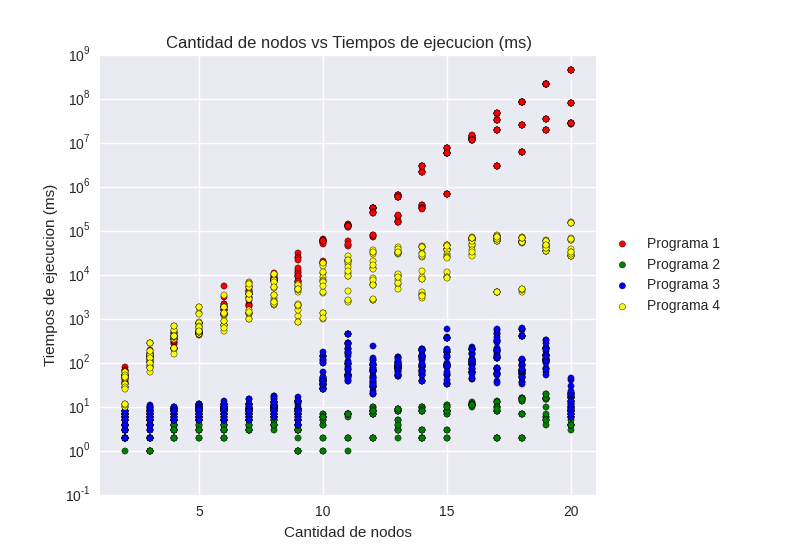
\includegraphics[width=\textwidth]{img/ejercicio5/tiempos_r1.png}
    \caption{Tiempos de ejecución en el rango 1. Programas 1, 2, 3 y 4}
    \label{fig: ej5_tiempos_r1}
  \end{center}
\end{figure}

\par En la figura \ref{fig: ej5_tiempos_r1} podemos ver los resultados del experimento. Notamos cláramente como el programa 1 se posiciona por encima del resto. Vemos también como el programa 4, en un primer momento mantiene tiempos similares. Esto se lo adjudicamos al hecho de que, al ser una cantidad muy reducida de nodos, calcular las vecindades para distintos resultados de una heurística golosa puede ser igual a pasar por las distintas soluciones válidas del problema (que es justamente lo que realiza el programa 1). Luego, a partir de los 10 nodos, se ve como calcular las vecindades deja de ser tan significativo.

\par A pesar de que el programa 4 se basa en una heurística de búsqueda local, al igual que el programa 3, la diferencia es que el primero realiza una cantidad grande de soluciones golososas y esto le da una cantidad grande de tipos de solucones válidas. Al buscar las vecindades de estos diversos tipos, se recorren más instancias.

\par Por su parte los programas 2 y 3 en ningún momento manejan tiempos cercanos al programa 1. Este también es un factor importante para tener en cuenta al comparar la calidad de las soluciones. Igualmente, a continuación veremos si esto se mantiene para otros rangos.

\subsection{Análisis 2: Tiempos de ejecución en el rango 2}

\par En este caso, correremos los programas 2, 3 y 4. Partimos de \textit{cantidad de nodos} = 2 y llegaremos hasta 200. Mediremos los tiempos de ejecución y luego analizaremos los resultados obtenidos.

\par Esperamos ver que el programa 4 tenga tiempos de ejecución mucho mayores a los otros dos. También queremos ver si entre los programas 2 y 3 comienzan a marcarse diferencias, ya que en el rango 1 vimos que comenzaban a separarse, pero no definidamente.

\begin{figure}[H]
  \begin{center}
    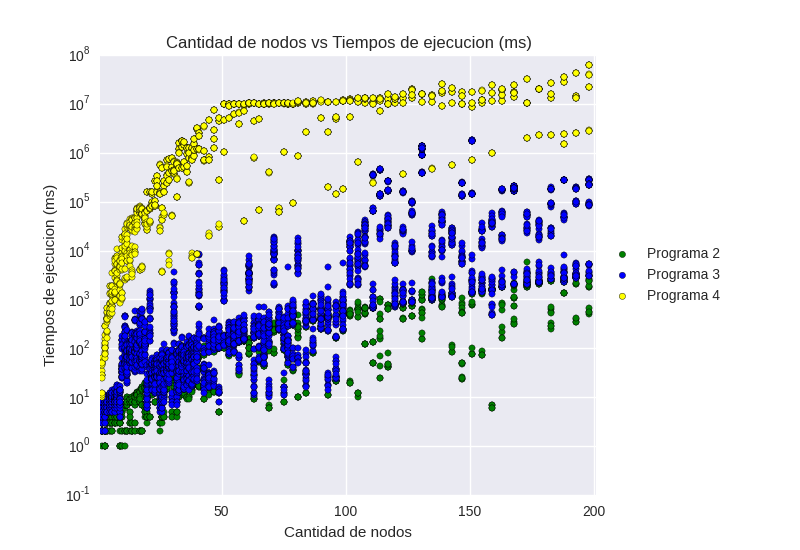
\includegraphics[width=\textwidth]{img/ejercicio5/tiempos_r2.png}
    \caption{Tiempos de ejecución en el rango 2. Programas 2, 3 y 4}
    \label{fig: ej5_tiempos_r2}
  \end{center}
\end{figure}

\par En la figura \ref{fig: ej5_tiempos_r2} podemos ver los resultados del experimento. Notamos como el programa 4 se desprende del resto y se mantiene en tiempos de ejecución muy por encima del resto. Pero un detalle interesante que notamos, es como a partir de los 50 nodos el tiempo se aplana bastante y deja de crecer de la manera en que venía haciéndolo. Esto se debe a que comienza a influir la cota de cantidad de ticks que se pone. A partir de una cierta cantidad de ticks de ejecución, el programa comienza a saltear nodos de inicio y termina más rápido la ejecución. Esto puede afectar mucho la calidad, pero de alguna forma debemos acotar los tiempos de ejecución.

\par Podemos ver como el programa 3 tiene algunos casos con tiempos cercanos al programa 2, mientras que en algunos casos estos tiempos se elevan. Esto se debe a que la heurística de búsqueda local depende mucho del caso de entrada. Si el caso de entrada puede aproximarse bien por la heurística golosa, luego se harán pocas mejoras y se obtendrá un tiempo cercano al programa 2 (que se basa justamente en una heurística golosa). También hay que tener en cuenta que entre los casos de experimentación hay casos inválidos. Esto hace que el programa 3, al llamar a la heurística golosa verifique que no le devolvió solución y no realice cambios (evitando así calcular las vecindades).

\subsection{Análisis 3: Tiempos de ejecución en el rango 3}

\par Para este último rango vamos a correr los programas 2 y 3. Partiremos de 2 nodos y llegaremos hasta 1000. Ahora sí vamos a exigir al programa 3, y esperamos que sus tiempos de ejecución se marquen muy por encima del programa 2. Pero nos interesa en particular ver qué tanta diferencia se ve entre ellos.

\begin{figure}[H]
  \begin{center}
    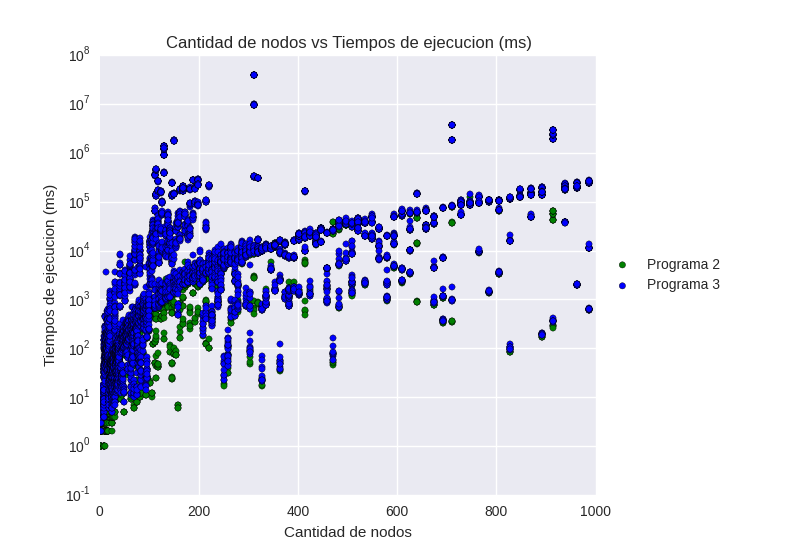
\includegraphics[width=\textwidth]{img/ejercicio5/tiempos_r3.png}
    \caption{Tiempos de ejecución en el rango 3. Programas 2 y 3}
    \label{fig: ej5_tiempos_r3}
  \end{center}
\end{figure}

\par En la figura \ref{fig: ej5_tiempos_r3} podemos ver los resultados del experiento. Lo primero que notamos es que no se ve tanta diferencia entre los programas como esperábamos. Si se ve que el programa 3 toma valores más dispersos en un primer momento, hasta aproximadamente 200 nodos. A partir de ahí, los valores del programa 3 se ven bastante cercanos a los del programa 2. Creemos que hay dos factores que pudieron ser muy importantes para que se de esto:

\begin{itemize}
	\item que el generador se haya mantenido en casos parecidos y por eso tengamos tiempos similares;
	\item que la heurística golosa haya sido bastante acertada y no se hagan muchos cambios en la búsqueda local.
\end{itemize}

\par Pero en principio, no notamos tanta diferencia entre los problemas. Tendremos que tener en cuenta esto a la hora de comparar calidad de las soluciones.


\subsection{Calidad de las soluciones}

\par Luego de haber analizado los tiempos de ejecución de los programas, vamos a ver la calidad de las soluciones comparándolas con el programa 1 (solución exacta). Para esto vamos a centrarnos en los resultados obtenidos en el rango 1, ya que era el único rango en el cuál corrimos el programa 1.

\par Vamos a presentar los resultados desde distintos enfoques para observar distintos detalles que creamos interesantes.

\subsubsection{Análisis 4: Porcentajes de error}

\par Lo primero que vamos a hacer es ver los porcentajes de error de cada caso, sacar promedios y ver cómo es su distribución.

\begin{table}[!htb]
	\caption{Porcentajes de error por programa}
	\label{tab: ej5_an4_porc_error}
	\begin{subtable}{.5\linewidth}
		\caption{Todos los casos.}
		\label{tab: ej5_an4_porc_error_todos}
		\centering
		\begin{tabular}{|C{2cm}|C{3.5cm}|}
			\hline
			Programa & Promedio de error \\
			\hline
			2 & 46.88 \% \\
			3 & 45.35 \% \\
			4 & 12.06 \% \\
			\hline
		\end{tabular}
	\end{subtable}
	\begin{subtable}{.5\linewidth}
		\centering
		\caption{Casos con solución válida.}
		\label{tab: ej5_an4_porc_error_validos}
		\begin{tabular}{|C{2cm}|C{3.5cm}|}
			\hline
			Programa & Promedio de error \\
			\hline
			2 & 48.14 \% \\
			3 & 46.58 \% \\
			4 & 12.38 \% \\
			\hline
		\end{tabular}
	\end{subtable}
\end{table}

\par En el cuadro \ref{tab: ej5_an4_porc_error} podemos ver los promedios de los porcentajes de error de cada programa. En los cuadro \ref{tab: ej5_an4_porc_error_validos} se encuentran diferenciados los casos válidos. Podemos ver que el programa 4 saca una gran diferencia en cuanto a calidad. Pasar de un error del 45\% a un error del 12\% es un cambio importante. Esto es un factor para contrastar con los resultados obtenidos en las mediciones de tiempos, donde el programa 4 marcó tiempos de ejecución notoriamente mayores a los de los programas 2 y 3.

\par Para ver más en detalle estos valores, en la figura \ref{fig: ej5_calidad_distr_porc} podemos ver la distribución de estos porcentajes. Viendo este gráfico reafirmamos la ventaja, en cuanto a calidad, del programa 4 por sobre el resto. Podemos ver que la mayor parte de sus porcentajes se encuentran muy cerca del cero, mientras que en los otros programas los porcentajes de error se distribuyen bastante más, posicionándose principalmente cerca del 50\%.

\begin{figure}[H]
  \begin{center}
    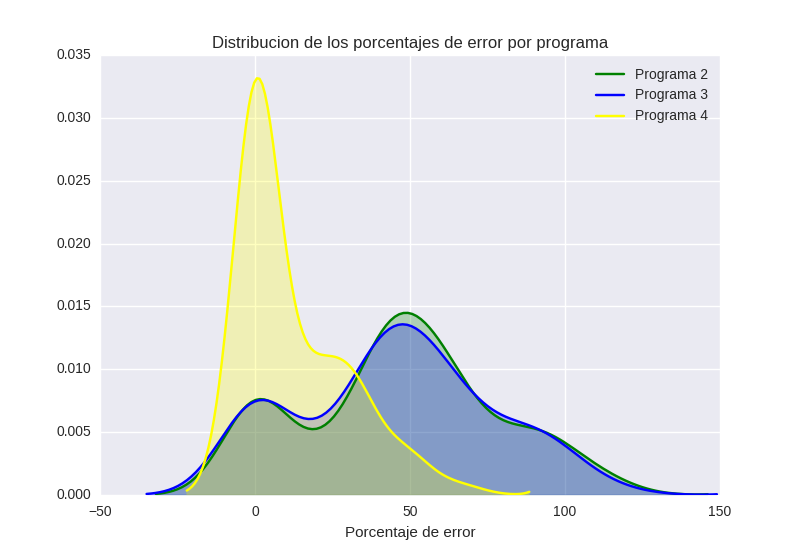
\includegraphics[width=\textwidth]{img/ejercicio5/calidad_distribuciones_error.png}
    \caption{Distribución de porcentajes de error por programa.}
    \label{fig: ej5_calidad_distr_porc}
  \end{center}
\end{figure}

\subsubsection{Análisis 5: Relación Tiempos-Calidad}

\par Luego de haber analizado la calidad de las soluciones brindadas por cada programa, nos vemos en la obligación de contrastar estos datos con los datos obtenidos en los experimentos previos. Para eso, vamos a definir una relación entre el tiempo de ejecución y el error de la solución final y veremos qué podemos ver a partir de esto.

\begin{figure}[H]
  \begin{center}
    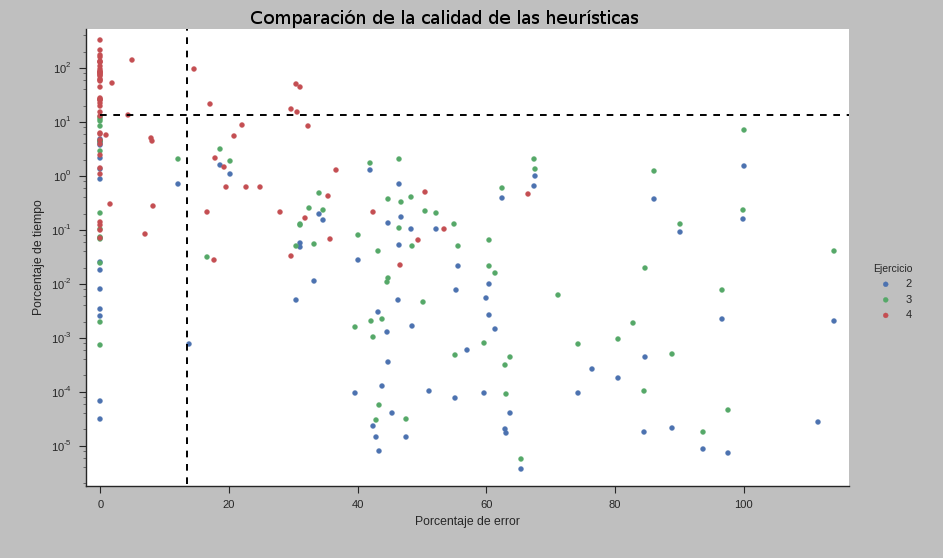
\includegraphics[width=\textwidth]{img/ejercicio5/relacion_tiempo_calidad.png}
    \caption{Gr\'afico que muestra la relaci\'on entre calidad y tiempo.}
    \label{fig: ej5_relacion_tiempo_calidad}
  \end{center}
\end{figure}
En la figura de arriba la l\'inea punteada vertical representa la media de los tiempos de nuestros experimentos mientras que la l\'inea punteada horizontal muestra la media de los errores con respecto a la soluci\'on exacta.
En la figura se puede ver que en el cuadrante que est\'a a la izquierda de la media de error y por encima de la media de tiempos predomina el GRASP, lo cual quiere decir que si uno cuenta con mucho tiempo y quiere una muy buena soluci\'on puede usar esa heur\'istica. En el cuadrante inferior derecho predominan el algoritmo goloso y la b\'usqueda local. ESto nos quiere decir que son soluciones econ\'omicas en cuanto a tiempo pero no muy buenas en cuanto a la calidad de la soluci\'on. En el cuadrante que se encuentra a la izquierda de la media de error y debajo de la media de tiempos predomina (pero no en demas\'ia) el GRASP. En el cuadrante restante hay algunos casos de GRASP pero son outliers.\\
La conclusi\'on que podemos sacar de este gr\'afico es que si se prefiere que la soluci\'on sea buena requiere mucho tiempo de procesamiento, en cambio si se necesita una soluci\'on r\'apida pero sin importar cuanto difiere de la \'optima se pueden usar las otras dos heur\'isticas.